\section{Diagrama de Atividades}

O diagrama de atividades permite modelar o comportamento do sistema, incluindo a sequência e as condições de execução de ações. Designa-se ações por unidades de comportamento do sistema e uma atividade por ações complexas que podem ser divididas em sequências de outras ações. As atividades podem advir:

\begin{itemize}
	\item Um caso de uso;
	\item Uma operação de uma classe;
	\item Um grupo de caso de uso relacionados entre si;
	\item Uma parte de uma atividade de mais alto nível;
\end{itemize}

\par Através dos diagramas de atividades a seguir representados, podemos ilustrar e entender melhor o fluxo de trabalho entre o \textit{user} e o sistema, assim como melhor entender a lógica do funcionamento do mesmo.

\newpage

\subsection{\labeltext[Diagrama de Atividades - Aluno]{Diagrama de Atividades - Aluno}{er:24}}

\begin{figure}[H]
	\centering
	\includegraphics[width=0.8\linewidth]{./img/Diagramas\_A/DA\_Aluno.jpg}  % largura percentual 
	\caption{\ref{er:24}}
	\label{fig:chap240}
\end{figure}

Pelo diagrama acima apresentado, podemos ver que o utilizador pode utilizar o sistema com ou sem login, porém apenas com o login executado é possivel ao mesmo usufruir de todas as vantágens do web-service. O mesmo é aplicado a todos os outros users, apenas com o login é possivel desbloquear todas as funcionalidades disponiveis.
No caso do utilizador podemos ver que as opções são maioritáriamente de consulta, permitindo ao mesmo fazer uma gestão pessoal dos livros requisitados, coimas e ver todos os livros disponiveis.
O utilizador, enquanto aluno, pode, dentro de todos estes campos, realizar ações mais aprofundadas como a realizar a requisição de um determinado livro, e anular ou alterar a data da mesma até 24horas antes da data de levantamento e fazer o pagamento de multas.
A devolução do exemplar é feita de forma fisica, e é registada pelo funcionario ou admin.

\newpage

%DA_Func
\subsection{\labeltext[Diagrama de Atividades - Funcionário]{Diagrama de Atividades - Funcionário}{er:241}}

\begin{figure}[H]
	\centering
	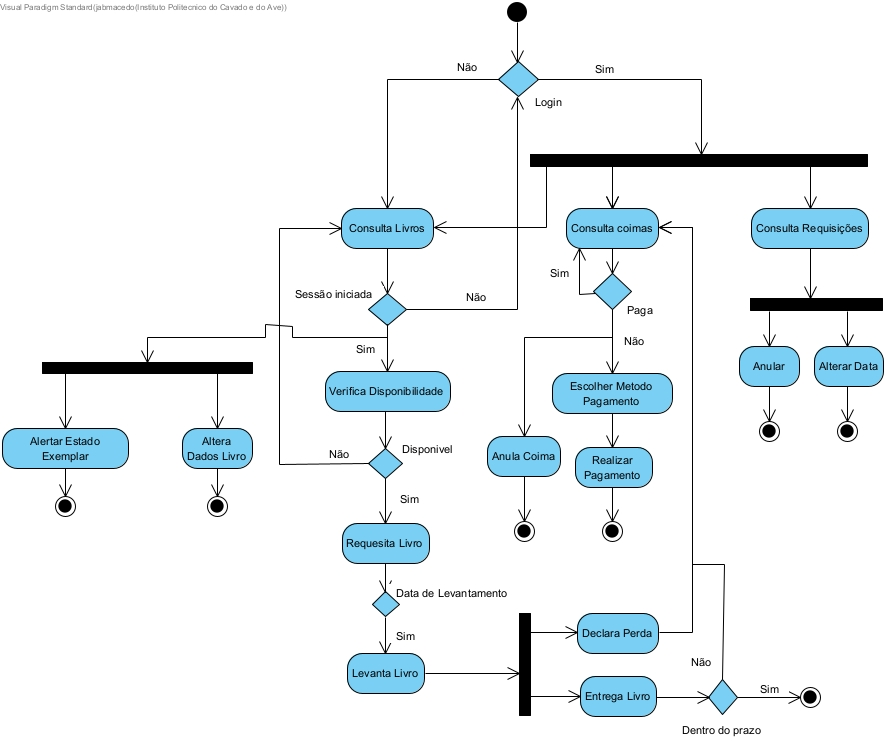
\includegraphics[width=1\linewidth]{./img/Diagramas_A/DA_Funcionario.jpg}  % largura percentual 
	\caption{\ref{er:241}}
	\label{fig:chap241}
\end{figure}

Com base no diagrama de atividade do funcionário, presente acima, é possivel observar que o mesmo possui um esquema identico ao do utilizador com apenas algumas adições e ligeiras alterações.
Um bom exemplo de uma alteração é quando observamos a consulta de requisições, já não sendo necessário o prazo de até 24h.
Quanto a funcionalidades adicionais, as principais são relativas aos exemplares/livros, o funcionario pode alertar o admin quanto ao estado de um determinado exemplar para que o admin possa proceder quanto ao tratamento dessa informação da melhor forma, e pode também alterar certos dados do livro, como o titulo, descrição, entre outros.
\newpage

%DA_Admin
\subsection{\labeltext[Diagrama de Atividades - Administrador]{Diagrama de Atividades - Administrador}{er:242}}

\begin{figure}[H]
	\centering
	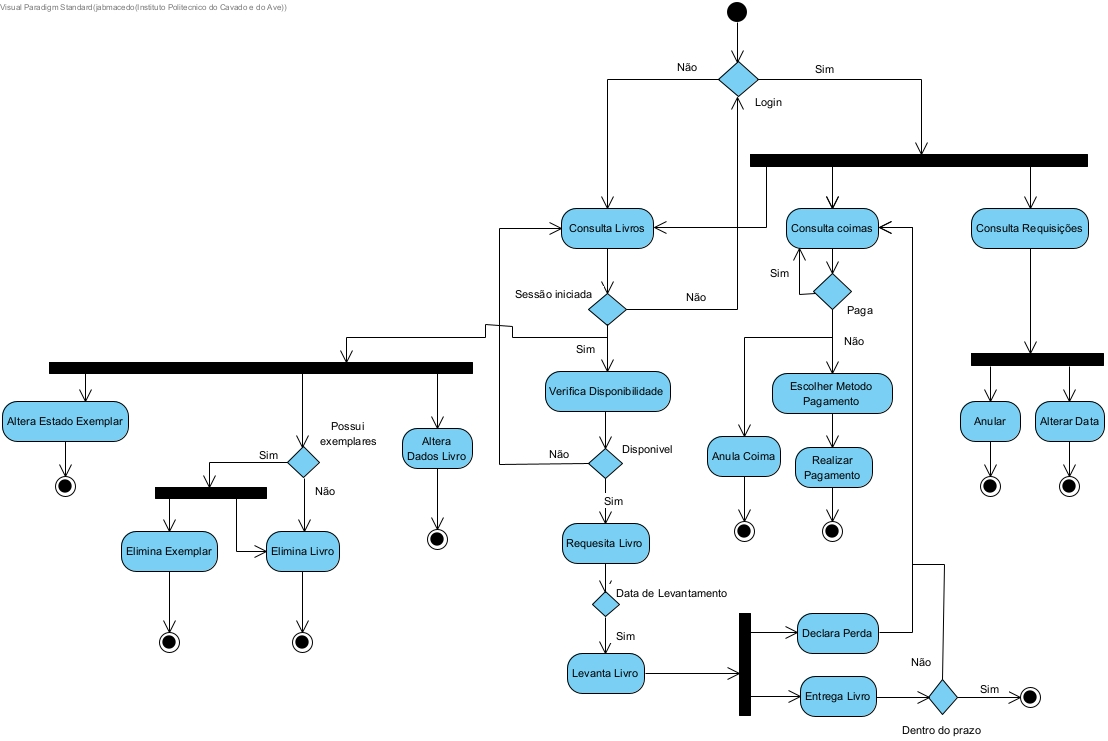
\includegraphics[width=1\linewidth]{./img/Diagramas_A/DA_Admin.jpg}  % largura percentual 
	\caption{\ref{er:242}}
	\label{fig:chap242}
\end{figure}

Como era de esperar, o administrador da biblioteca, ou qualquer user com o tipo admin, ter acesso ao maior numero de funcionalidades e maior liberdade de manipulação de dados.
O Admin pode realizar a eliminação de exemplares e livros, alterações manuais aos seus estados, assim como anular coimas, anular/alterar requisições, entre outras.
A maioria das funcionalidades são identicas para todos os utilizadores como o registo de uma requisição, a forma como as mesmas são geridas, consulta dos livros, consulta das coimas e a gestão das mesmas, sendo apenas aplicadas determinadas regras de negócio que permitem a existencia de uma hierarquia de ações que podem, se mal geridas, corromper todo o sistema.
\newpage


